\section{Results, Evaluation and Experiments}
In this section, we will discuss the results obtained in multiple conditions. Those data were recorded using ROSBag and were parsed using the ROSBag python module.
We provide a jupyter notebook in the repository that facilitates drawing all the relevant graphs with a convenient way of storing all the parsed bags inside a pickle file.

\subsection{Compensation for drag}
In the first experiment, we will justify the need for a air drag compensation term. 
The velocity field we use in the circular velocity field based on \cite{mcinnes2003velocity}.
\subsubsection{Experience without drag compensation}
\begin{figure*}[h!]
   \centering
   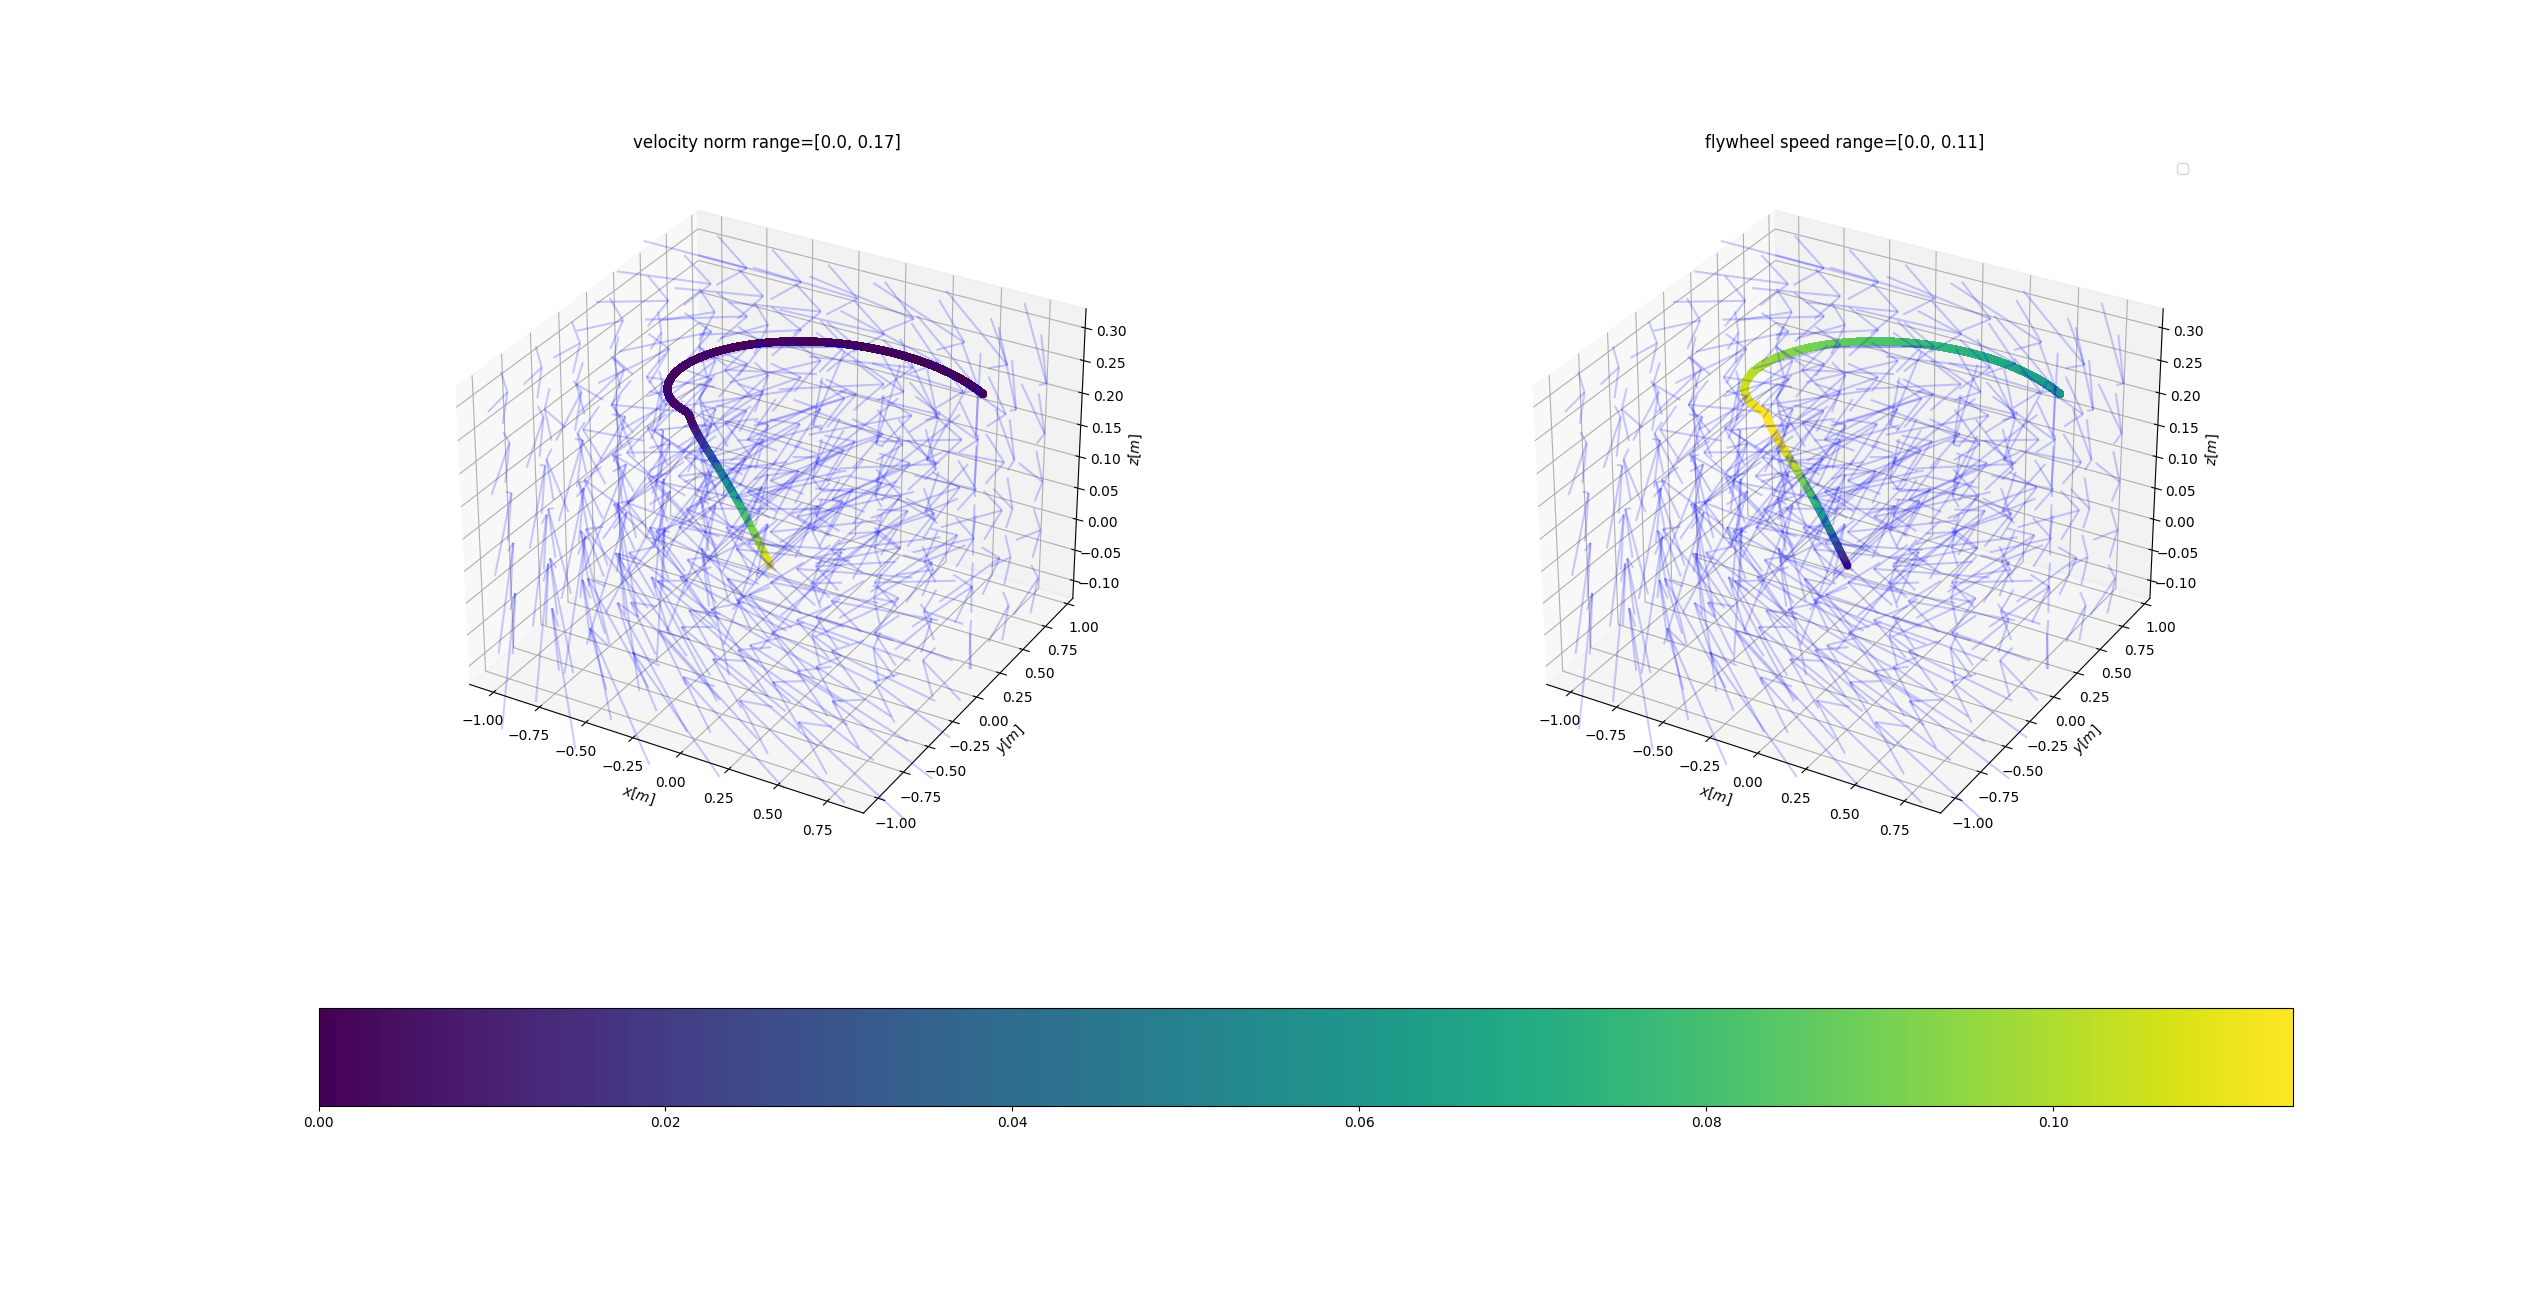
\includegraphics[width=\linewidth]{Images/python-noforcecomp.png}
   \caption{trajectory and mechanical energy without force compensation }
   \label{fig:pythonnocomp}
\end{figure*}
On the both of figure \ref{fig:pythonnocomp}, we can see the trajectory of the quadcopter, the left scatter plot of the trajectory is colored according to the
translational velocity the quadcopter while the right scatter plot is colored according to the angular velocity of the fictitious flywheel.
On both subplot, the quiver plot represents the desired velocity field
We can see that when we do not introduce a drag force compensation, the quad translational velocity goes to zero. 
This is explained by the fact by the quadcopter thrust given by PVFC has a too low amplitude to compensate the drag force, the quad decelerate.
The amplitude of the flywheel velocity is not affected by this drag because we defined a perfect no friction flywheel.\\
These subplots are useful to observe how energy is being transfered between the fictitious flywheel and the quadcopter. 
We can see that as expected from equation \ref{eqn:vfly}, the faster the quad is going the slower the fictitious flywheel is spinning.

\begin{figure}[h!]
   \centering
   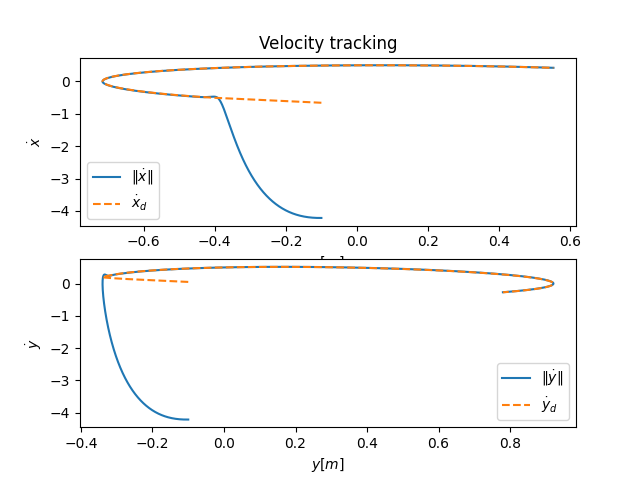
\includegraphics[width=\linewidth]{Images/velocitytrackingpythonnocomp.png}
   \caption{Trajectory tracking without force compensation }
   \label{fig:trajtracknocomp}
\end{figure}

Despite the total stop, we can see from the figure \ref{fig:trajtracknocomp} that the field is accuratly followed
\subsubsection{Experience with drag compensation}
This experiment is the same as the last one except that we add to the desired pvfc thrust output the compensation term $\tau_{comp} = C\cdot \dot{q}$ 
where $C$ is current translational coriolis matrix and $\dot{q}$ is the current translational velocity of the quadcopter.
\begin{figure*}[h!]
   \centering
   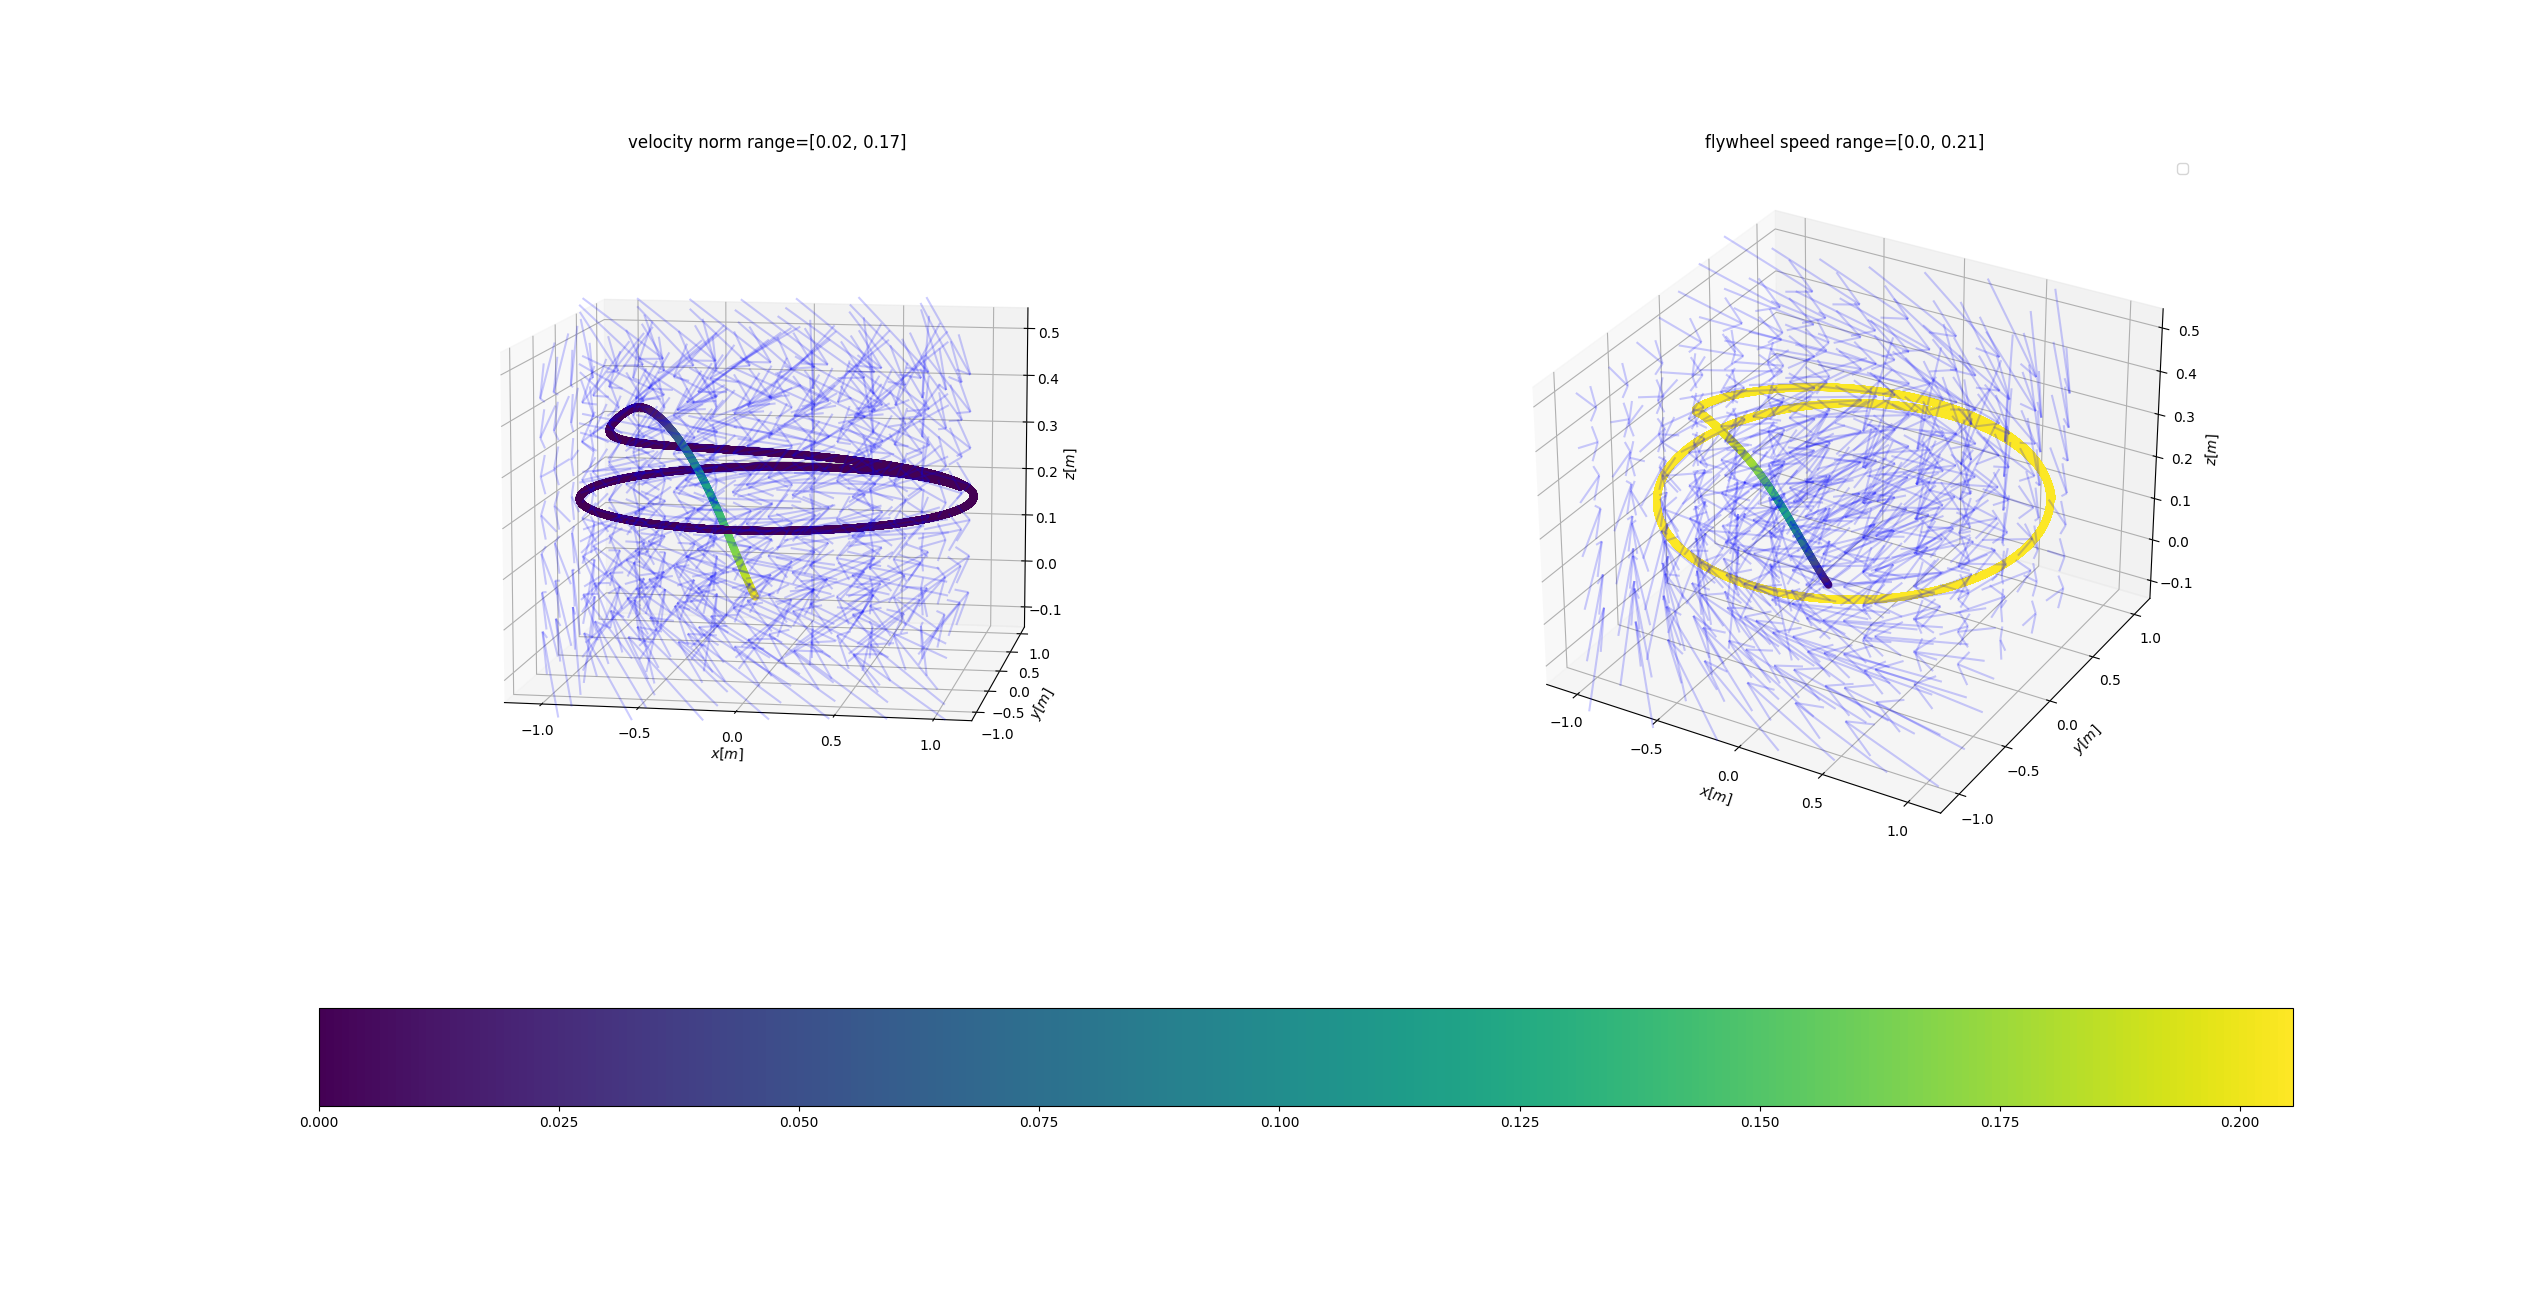
\includegraphics[width=\linewidth]{Images/python-forcecomp.png}
   \caption{trajectory and mechanical energy with force compensation }
   \label{fig:pythoncomp}
\end{figure*}
We can see in figure \ref{fig:pythoncomp} that introducing this force compensation allows the quad to continue moving despite drag forces. 
However, use such compensation slightly decreases the precision of the velocity field tracking (figure \ref{fig:trajtrackcomp}). It is not clear why this is happening.
\begin{figure}[h!]
   \centering
   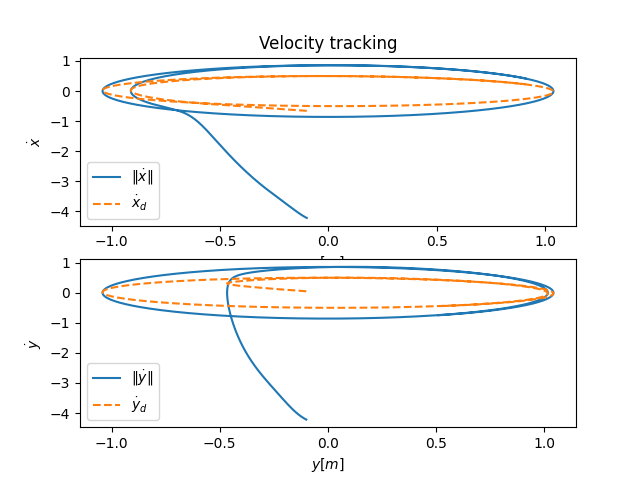
\includegraphics[width=\linewidth]{Images/velocitytrackingpythoncomp.png}
   \caption{Trajectory tracking with force compensation }
   \label{fig:trajtrackcomp}
\end{figure}

\subsection{No drag forces}
In this second experiment, we remove the drag forces from the dynamics (we set the drag coefficients to 0).
We can see in the figure \ref{fig:pythonnodrag} that when far away from the desired path, the translational speed of the quadcopter is high while the rotation speed of the flywheel is low.
This is happening because of the way the veloicty field is constructed in equation \ref{eqn:circularfieldcons}, 
the magnitude of the tangential component is constant but the magnitude of the normal component is proportional to the distance between the quad and the closest point in the circle.
We can observe how energy is being traded between the quad and the flywheel when the quad approaches the desired path.
\begin{figure*}[h!]
   \centering
   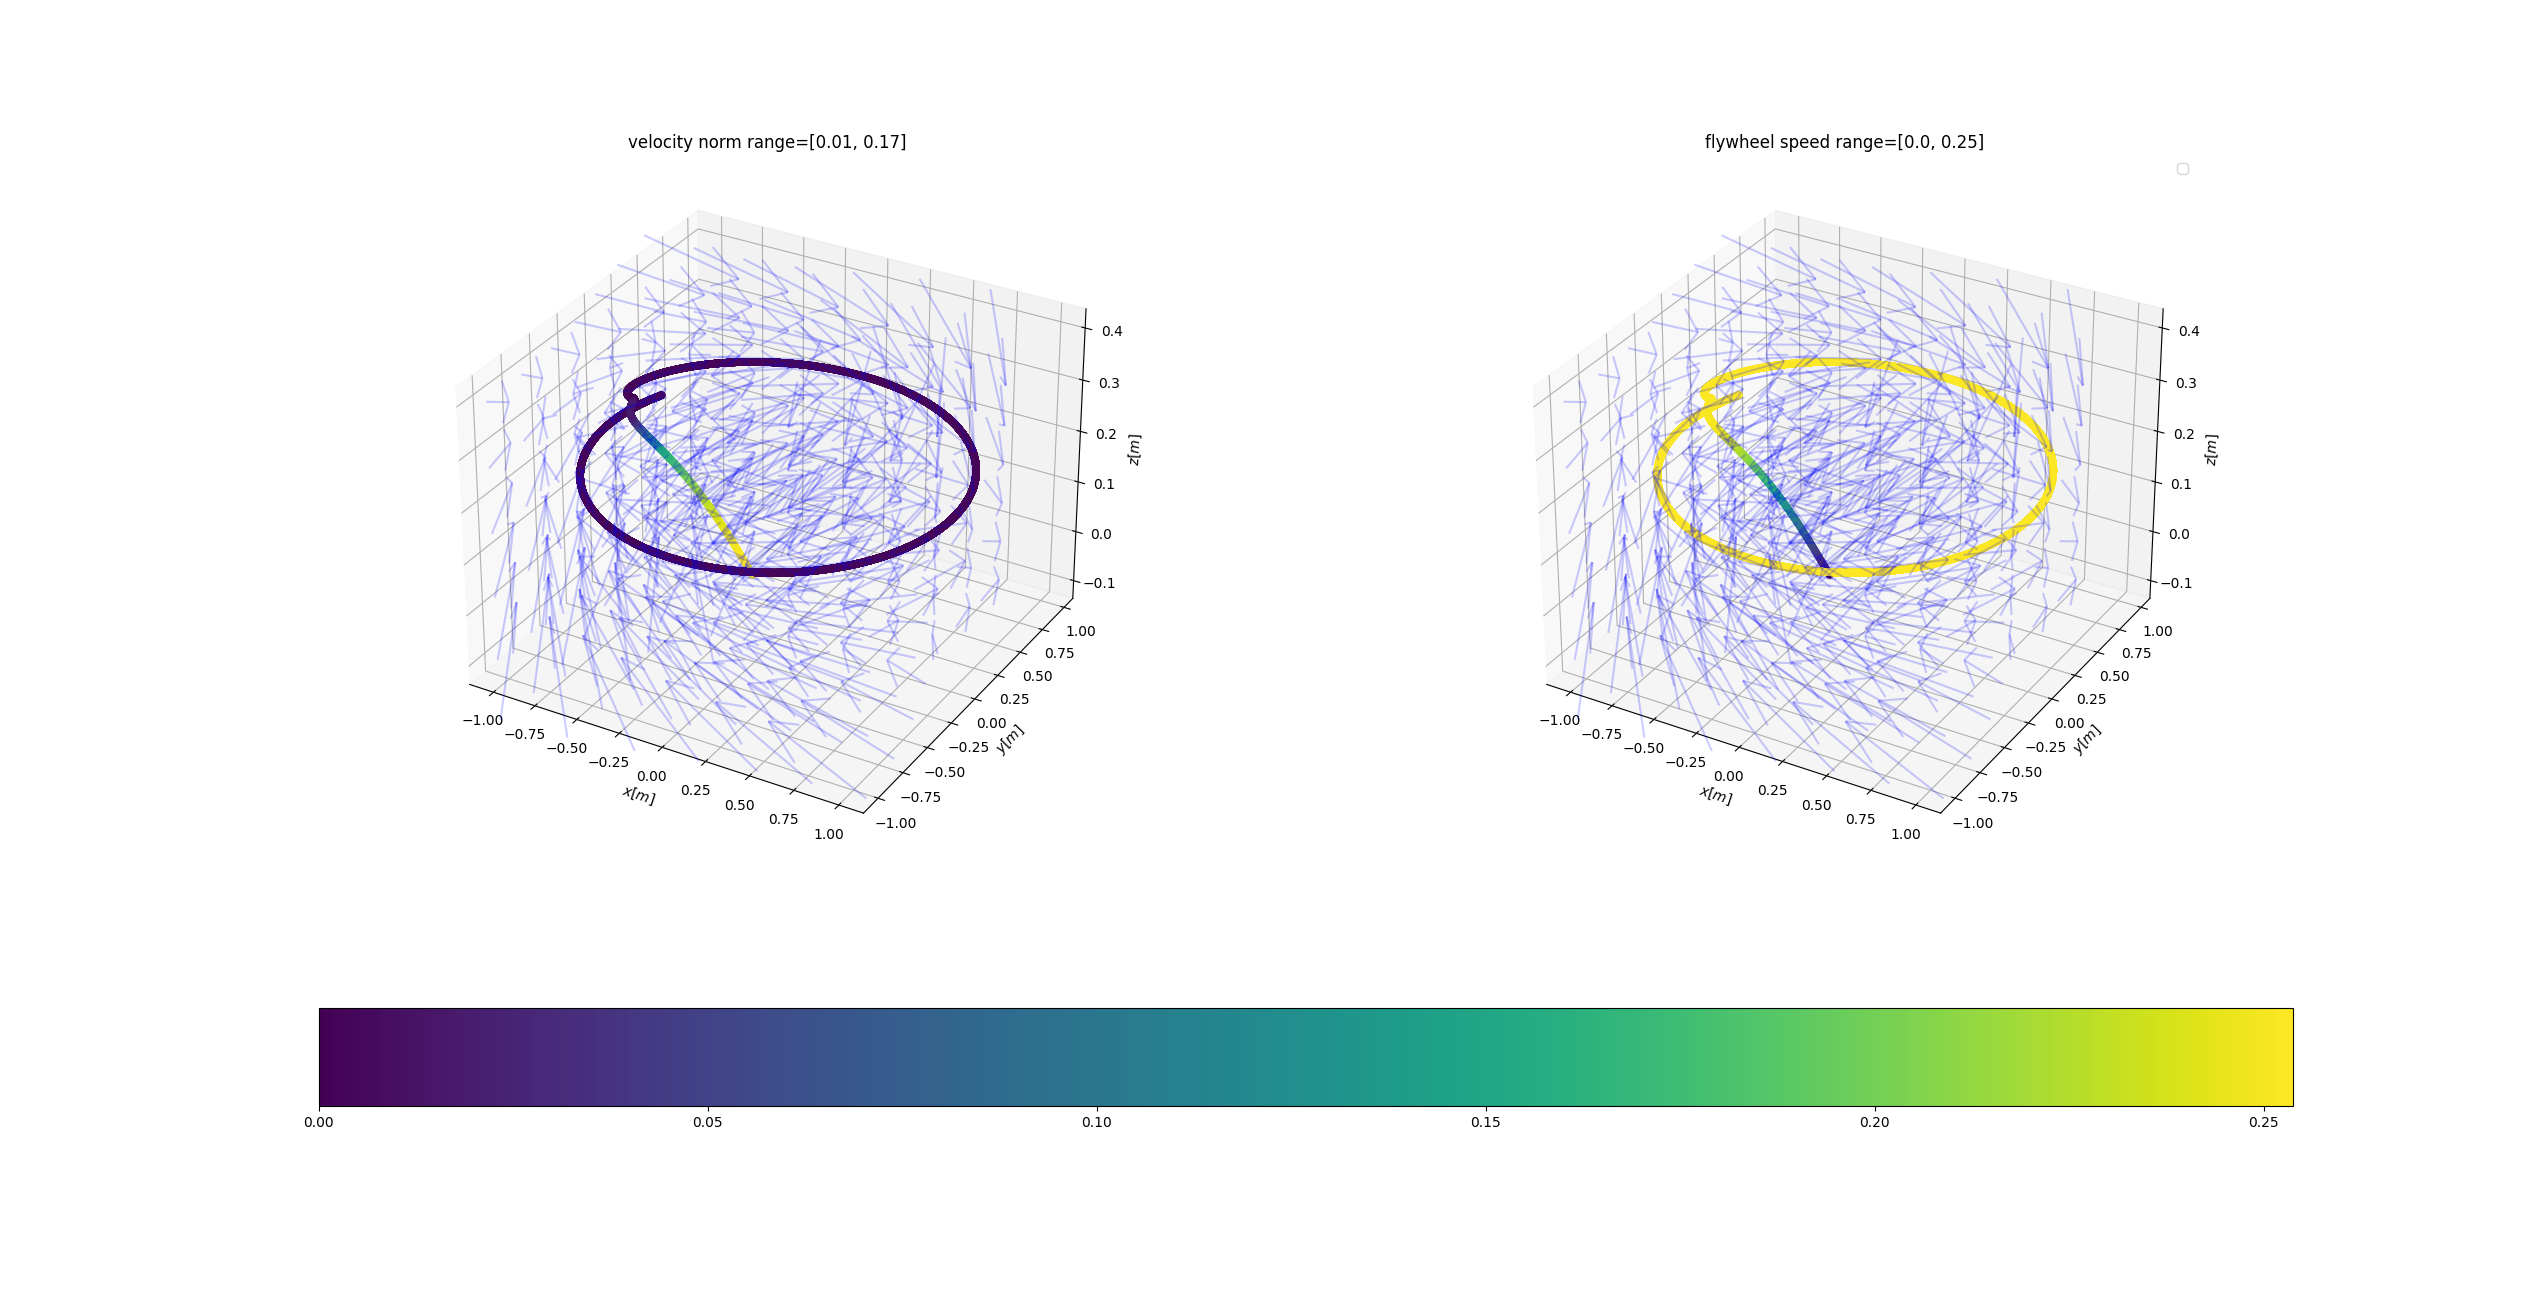
\includegraphics[width=\linewidth]{Images/python-nodrag.png}
   \caption{trajectory and mechanical energy without drag }
   \label{fig:pythonnodrag}
\end{figure*}
It should also be noted that the desired path is exactly followed in opposition to the last experiment with drag compensation (see figure \ref{fig:trajtracknodrag})
\begin{figure}[h!]
   \centering
   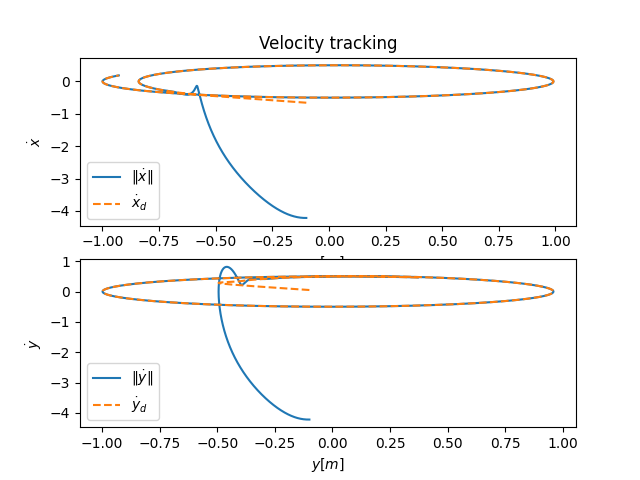
\includegraphics[width=\linewidth]{Images/velocitytrackingpythonnodrag.png}
   \caption{Trajectory tracking without drag}
   \label{fig:trajtracknodrag}
\end{figure}
We explained in section 3 that PVFC has interesting properties regarding the velocity tracking error (eq \ref{alphaerror}). 
The author in \cite{li1999passive} explains that When no external forces are applied on the quadcopter, $\alpha$ should approach $\beta^2 = \frac{\text{augmented mechanical energy}}{\text{augmented desired mechanical energy}}$.\\
In addition, when $\alpha$ approach $\beta$, the $alpha$ error should approach 0.

\begin{figure}[h!]
   \centering
   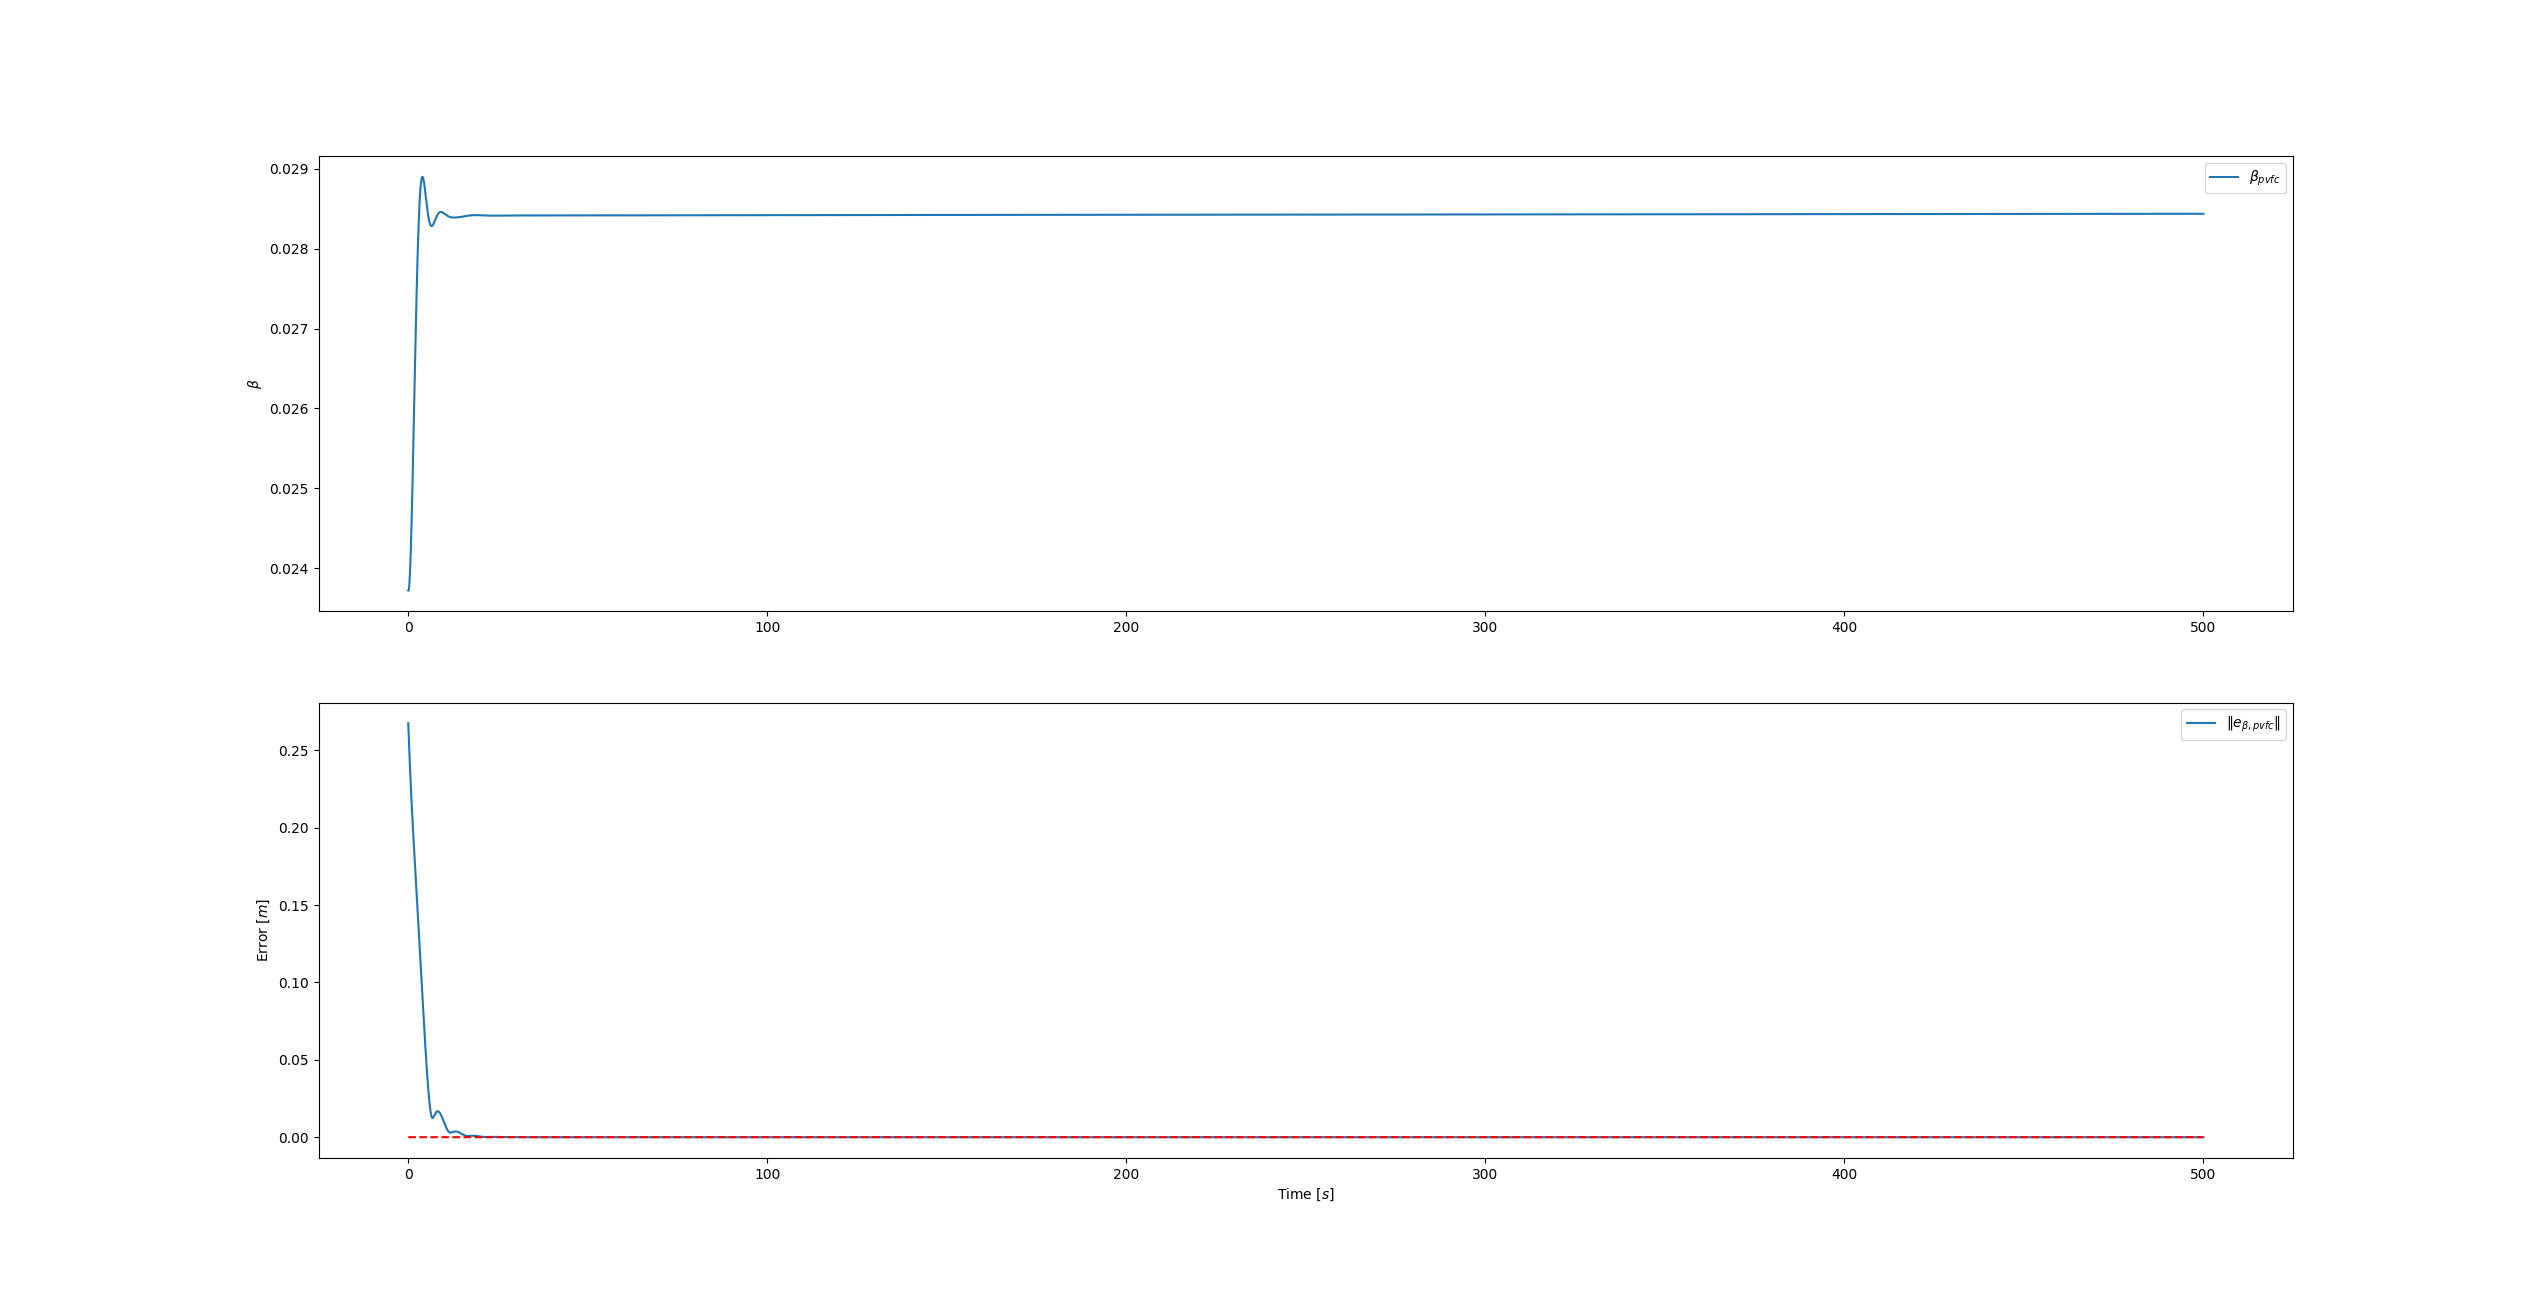
\includegraphics[width=\linewidth, scale=1.5]{Images/betaerrornodrag.png}
   \caption{Beta error without drag}
   \label{fig:betaerrornodrag}
\end{figure}
By design, the augmented desired mechanical energy of the system is always equal to $\bar{E}$, and we compute the augmented mechanical energy such that:\\ $\text{augmented mechanical energy} = \frac{1}{2}m_b\lVert\dot{q}\rVert + \frac{1}{2}m_{fly}\lVert\dot{q}_{fly}\rVert $
We successfully reproduced the results of \cite{li1999passive} for the $\beta$ error on a circular velocity field. We can see in figure \ref{fig:betaerrornodrag} that $\beta$ converges and the $\beta$ error converges to 0.

\subsection{No drag forces with force wrench}
The third experiment is done in 3 phases: In the first one we let the quad follow the circular field for 120 seconds, 
then we apply an external force on the quad in the $-\hat{y}$ direction for 10 seconds,
and finaly we let the quad follow the desired field for 120 seconds.
\begin{figure*}[h!]
   \centering
   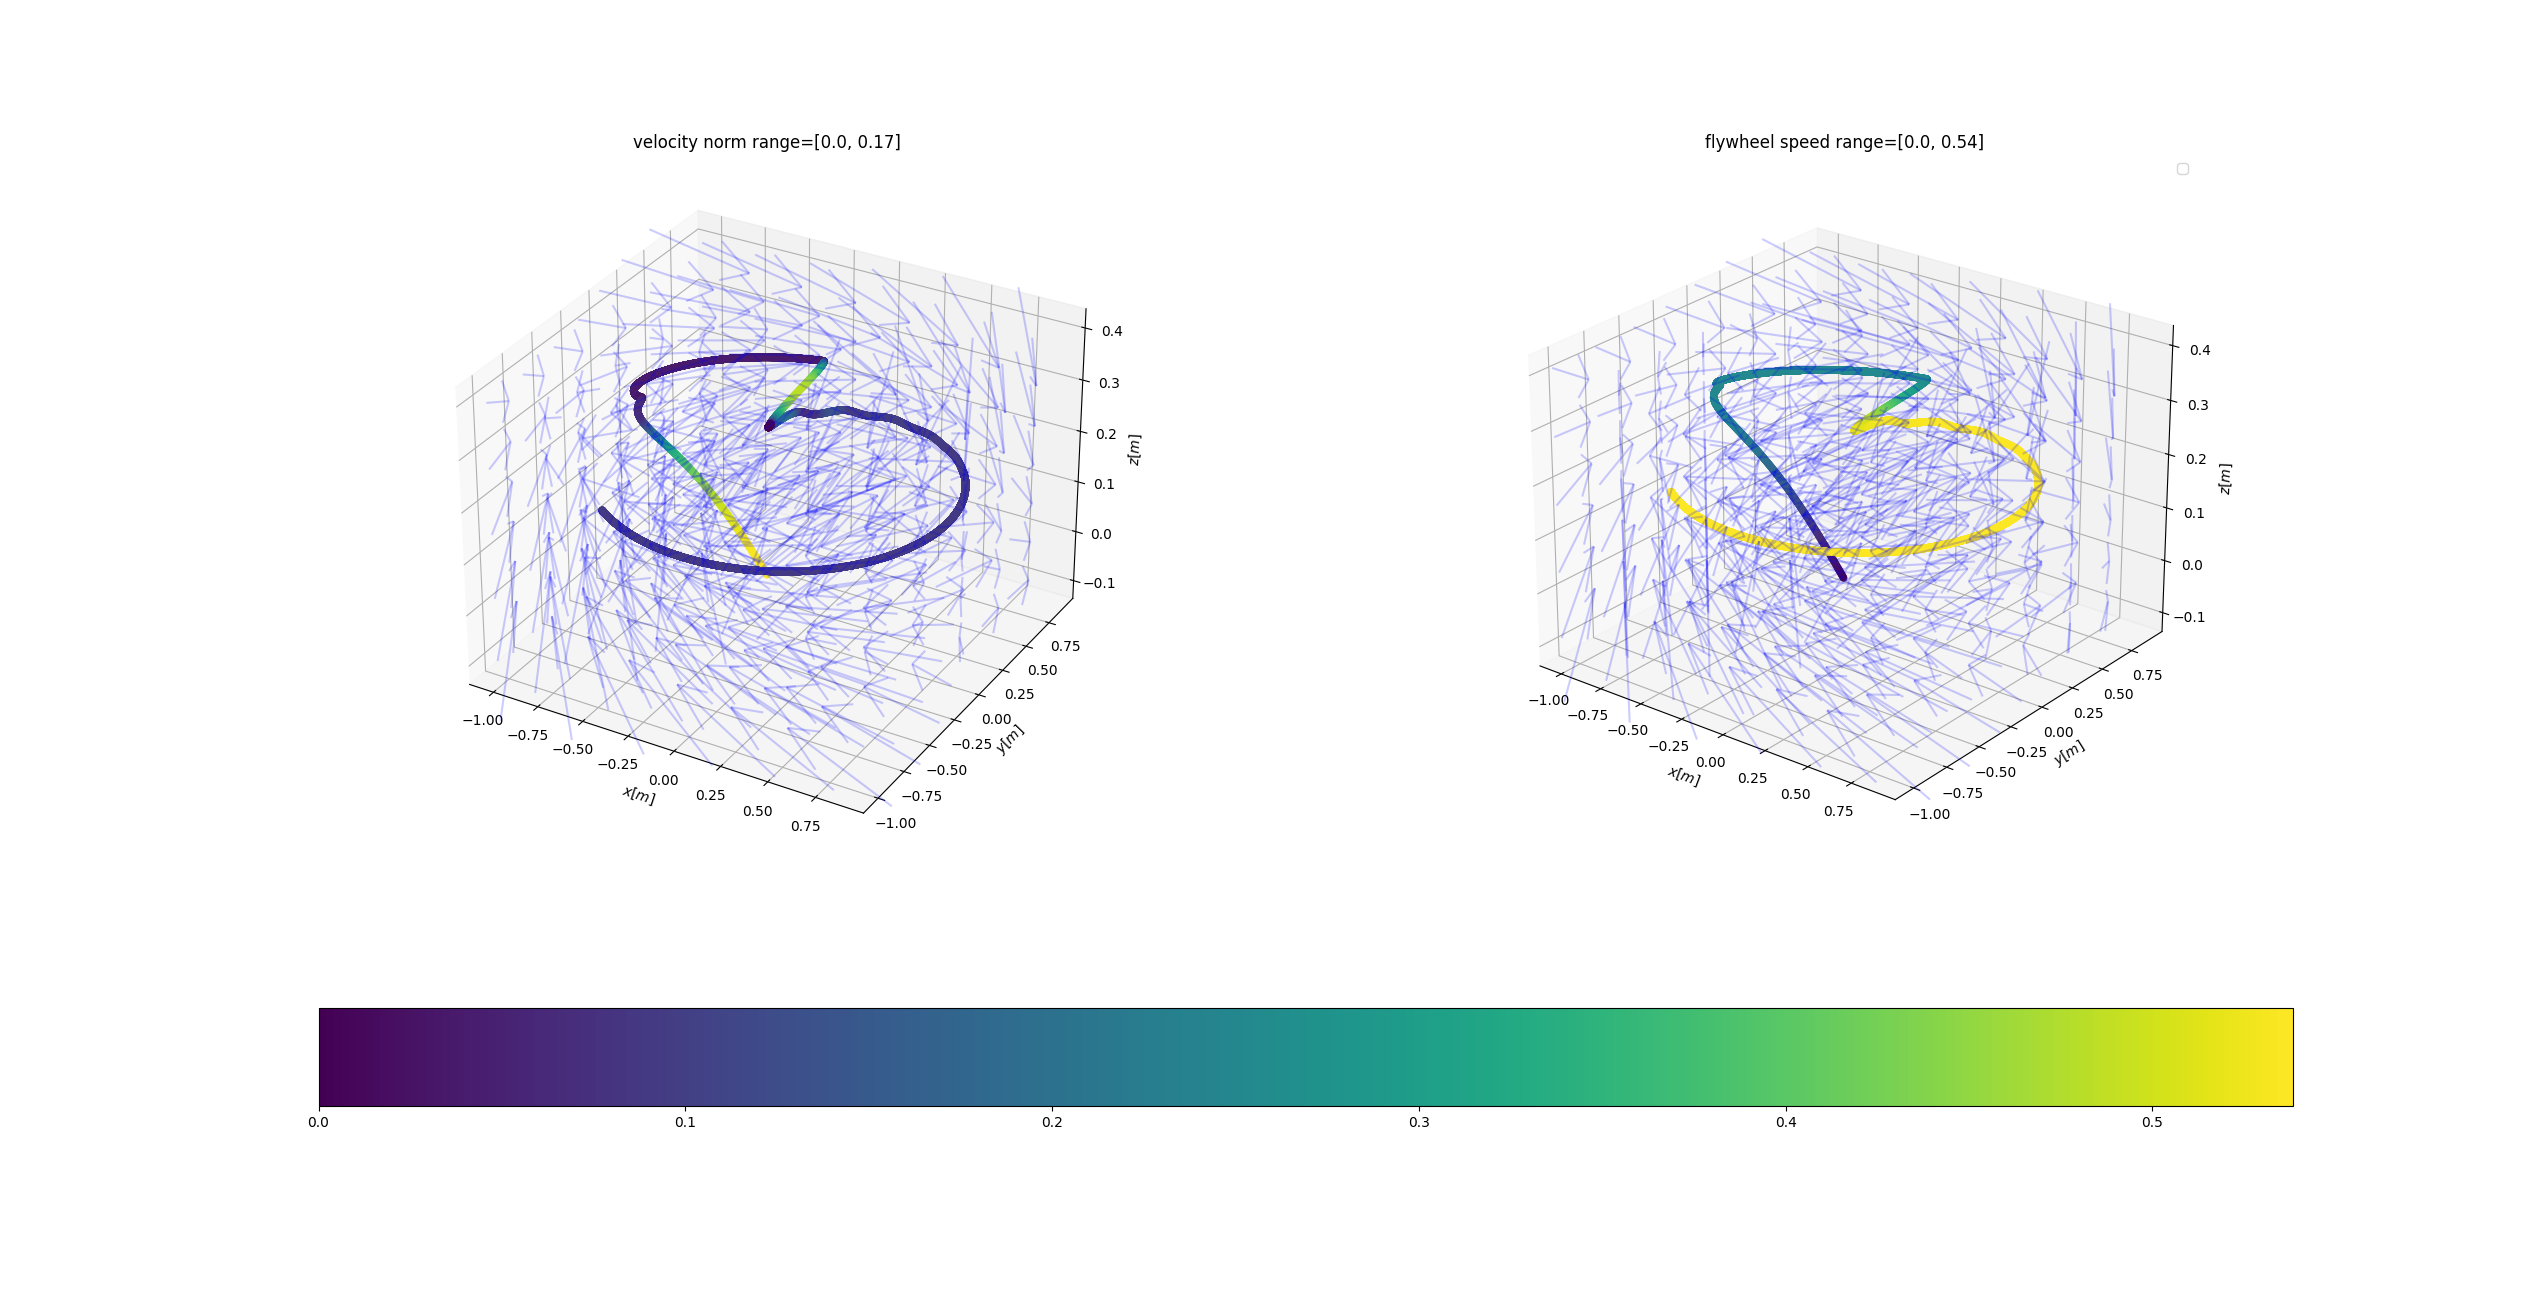
\includegraphics[width=\linewidth]{Images/python-nodrag-wrench.png}
   \caption{trajectory and mechanical energy without drag and with wrench }
   \label{fig:pythonnodragwrench}
\end{figure*}
The passivity properties of PVFC are well shown in figure \ref{fig:pythonnodragwrench}. We can see how the quadcopter is trading energy with the environement and dissipating the work of the wrench inside the augmented system.
This experiment also exemplify well the advantage of using velocity field instead of a traditional trajectory following based controller:
\begin{figure}[h!]
   \centering
   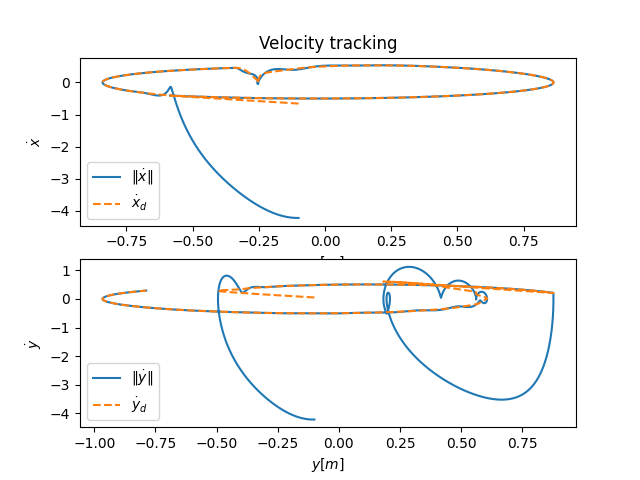
\includegraphics[width=\linewidth]{Images/velocitytrackingpythonnodragwrench.png}
   \caption{Trajectory tracking without drag with wrench}
   \label{fig:trajtracknodragwrench}
\end{figure}
The radial reduction that could have occured in figure \ref{fig:trajtracknodragwrench} could have been a big issue in a task such as countour following where following the countour is more important than following a trajectory.
In the contrary, figure \ref{fig:trajtracknodragwrench} shows that when external forces are applied, we are able to go back to the desired circular path without radial reduction.
In addition, we can observe what happens to the $\beta$ error when wrench is applied:
\begin{figure}[h!]
   \centering
   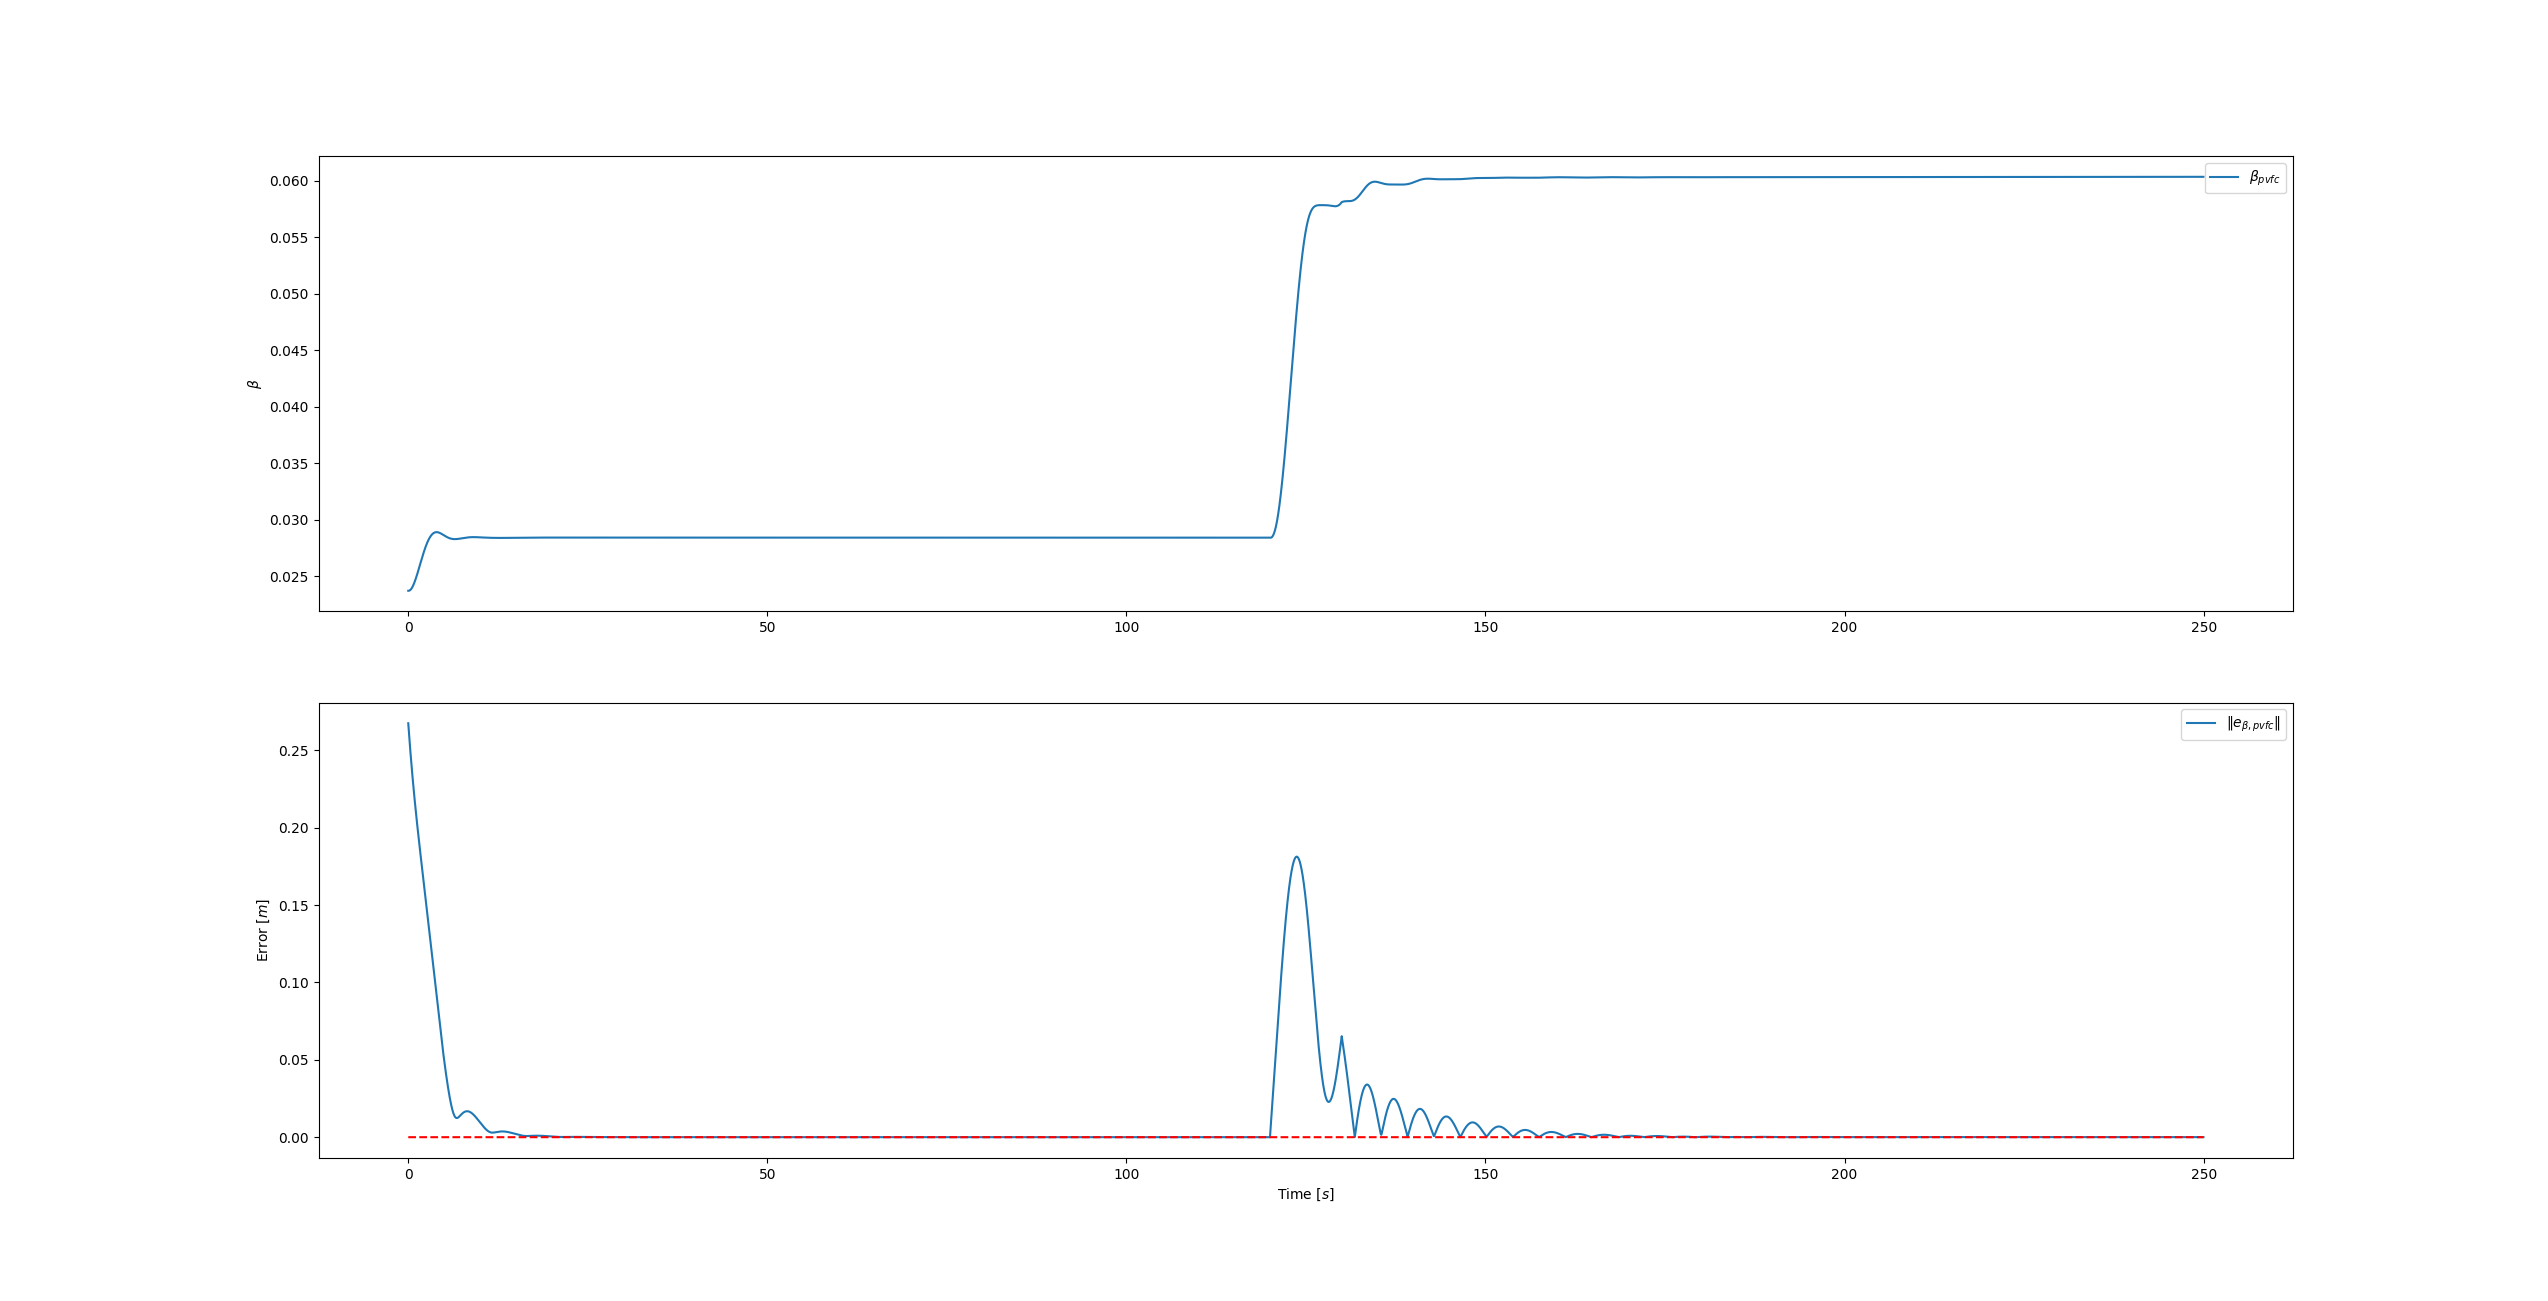
\includegraphics[width=\linewidth, scale=1.5]{Images/betaerrornodragwrench.png}
   \caption{Beta error without drag with wrench}
   \label{fig:betaerrornodragwrench}
\end{figure}
We can see in figure \ref{fig:betaerrornodragwrench} that the $\beta$ error converges to 0 before a wrench is applied, 
then during the second phase, we can see a spike for both $\beta$ and $\beta$ error when a wrench is applied. This is expected since the wrench increases mechanical energy in the system. 
We can see how PVFC dissipates the external force and makes the $\beta$ error converge to 0 when no external force is applied in the last phase.

Now we are going to show experiments done on the Gazebo simulation
\subsection{Gusty world}

\subsection{Windy world}

\subsection{gamma analysis}

\subsection{Ebar analysis}



 \begin{itemize}
    \item Calibrate thrust
    \item  introduction of compensation terms for friction
    \item finetuning (Ax Ay Az). too high cause speed to diverge, too low the quad lose all its energy and stop. 
    \item beta error
    \item presents experiences in different worlds
    \item using wind world helped lead the way to understand the need for compensation
    \item Analyze Ebar, Gamma
 \end{itemize}
 \newpage
 
